\documentclass[a4paper,11pt]{article}

\usepackage{amsmath, amssymb, amstext, amsfonts, mathrsfs}


% \sffamily %schrift ohne Serifen

\usepackage[T1]{fontenc} 
% schriftencodierung f�r umlaute, trennung
% f\"ur Uni
\usepackage[latin1]{inputenc}
\usepackage{selinput}
% \usepackage[utf8x]{inputenc} 
\usepackage{bibgerm} 
% german bibliography
\usepackage[german]{babel}
%wichtig f�r deutschen Content
\usepackage{ucs}
%erweiterte UTF-8 Unterst�tzung
\usepackage{wrapfig} 
% Paket zur Positionierung einbinden
\usepackage{multirow}
% zusammenfassen von Tabellenzellen
% \usepackage{subscript}
% zum tiefstellen
\usepackage{lscape}
\usepackage{pdflscape}
% zum drehen der Seite
% \usepackage[super]{natbib}
\usepackage[square,sort,comma,numbers]{natbib}
% Erstellung es Literaturverzeichnisses
\usepackage{url}
% Umbruch f�r URL
\usepackage{pst-3dplot}
% f�r tex Grafiken n�tig
\usepackage{pstricks}
\usepackage{listings}
% f�r das einf�gen von Quelltext
\definecolor{codegray}{rgb}{0.92,0.92,0.92}
\lstset{basicstyle=\fontsize{9}{11}\selectfont\ttfamily, breaklines=true, backgroundcolor=\color{codegray}, numbers=left, numberstyle=\tiny, tabsize=4, language=java}
\definecolor{mymauve}{rgb}{0.58,0,0.82}
\definecolor{mygreen}{rgb}{0,0.6,0}
\lstset{
commentstyle=\color{mygreen},
keywordstyle=\color{mymauve},
language=Java,
stringstyle=\color{blue}
}


%Einstellungen f�r Quellcode
\usepackage[a4paper, left=3cm, right=2cm, top=2cm]{geometry}
% Formatierung R�nder
\usepackage[section]{placeins}
% f�r Floatbarriere
\usepackage{color}
\usepackage{colortbl}
%f�r die Verwendung von Farben

\clubpenalty = 10000 
\widowpenalty = 10000
\displaywidowpenalty = 10000
%Verhinderung von Hurenkindern und Schusterjungen
%10000 bedeutet die sie sollen kommplett vermieden werden

\title{Entwicklung einer Android-Applikation f�r die Alarmierung der Einsatzkr�fte der Freiwilligen Feuerwehren}

\author{Sebastian Rieger}

\pagenumbering{arabic}
%Seitenzahlen(arabische Zahlen)

\setlength{\parindent}{0.25cm} 
%Absatzeinzug �ndern in Zoll
\setlength{\parskip}{0.25cm}
%Absatzabstand
\linespread {1.5}
%Zeilenabstand

\usepackage{setspace}
\usepackage{hyperref}
%anklickbare Hyperlinks

%funktioniert nicht bei Fu�noten
\usepackage{graphicx}
\usepackage{graphics}
%f�r einbinden von Grafiken

\usepackage{framed}
%f�r Umrandung der Erkl�rung
\usepackage{acronym}
% f�r abk�rzungen
% \usepackage{PSTricks}
\usepackage{epstopdf}
% f�r eps bilder nutze pdflatex --shell-escape this.tex
\usepackage{amssymb}
% f�r mathematische Symbole

\usepackage{hyperref}
% klickbare links

% \usepackage{pdfpages}
\usepackage{rotating}
\usepackage{svg}
%%%%%%%%%%%%%%%%%%%%%%%%%%%%%%%%%%%%%%%%%%%%%%%%%%%%%%%%%%%%%%%%%%%%%%%%%%%%%%%%%%%%%%%%%%%%%%%%%%%%%
%% Angaben zur Arbeit
%%%%%%%%%%%%%%%%%%%%%%%%%%%%%%%%%%%%%%%%%%%%%%%%%%%%%%%%%%%%%%%%%%%%%%%%%%%%%%%

\newcommand{\Autor}{Sebastian Rieger}
\newcommand{\MatrikelNummer}{10286908}
\newcommand{\Kursbezeichnung}{TINF12B1}

\newcommand{\FirmenName}{PDV Systeme}
\newcommand{\FirmenStadt}{Erfurt}
\newcommand{\FirmenLogoDeckblatt}{{
\includegraphics[width=3cm]{Bilder/PDV-Systeme}}}

% Falls es kein Firmenlogo gibt:
%  \newcommand{\FirmenLogoDeckblatt}{}

\newcommand{\BetreuerFirma}{Dipl. -Witschaftsinform. (FH) Nico Kaiser}
\newcommand{\BetreuerDHBW}{Prof. Rolf Kruse}
\newcommand{\Titel}{Evaluation moderner Webtechnologien f�r die Entwicklung eines modularen Supportportals}
\newcommand{\AbgabeDatum}{01.03.2017}

\newcommand{\Dauer}{24 Wochen}

% \newcommand{\Abschluss}{Bachelor of Engineering}
\newcommand{\Abschluss}{Master of Science}

\newcommand{\Studiengang}{Angewandte Informatik}
% \newcommand{\Studiengang}{Angewandte Informatik}
\newcommand{\Was}{Master Projekt}

%%%%%%%%%%%%%%%%%%%%%%%%%%%%%%%%%%%%%%%%%%%%%%%%%%%%%%%%%%%%%%%%%%%%%%%%%%%%%%%%%%%%%%%%%%%%%%%%%%%%% 
%steuervariable
\usepackage{ifthen} %Package f�r if/else
\newboolean{bilder} %Deklaration
\setboolean{bilder}{true} %Zuweisung
% \setboolean{bilder}{false} %Zuweisung
%%%%%%%%%%%%%%%%%%%%%%%%%%%%%%%%%%%%%%%%%%%%%%%%%%%%%%%%%%%%%%%%%%%%%%%%%%%%%%%%%%%%%%%%%%%%%%%%%%%%%

\makeatletter
\newcommand\footnoteref[1]{\protected@xdef\@thefnmark{\ref{#1}}\@footnotemark}
\makeatother

\begin{document}

\begin{center}
\vspace*{-2cm}
\FirmenLogoDeckblatt\hfill
\includegraphics[width=4cm]{Bilder/logo_FHE}\\[1cm]
{\Huge \Titel}\\[2cm]
{\Huge\scshape \Was}\\[2cm]
% {\large f�r die Pr�fung zum}\\[0.5cm]
% {\Large \Abschluss}\\[0.5cm]
% {\large des Studienganges \Studiengang}\\[0.5cm]
{\large \Studiengang}\\[0.5cm]
{\large an der}\\[0.5cm]
{\large Fachhochschule Erfurt}\\[0.5cm]
{\large von}\\[0.5cm]
{\large\bfseries \Autor}\\[1cm]
{\large Abgabedatum \AbgabeDatum}
\vfill
\end{center}
\begin{tabular}{l@{\hspace{1cm}}l}
Bearbeitungszeitraum             & \Dauer                       \\
Matrikelnummer                   & \MatrikelNummer              \\
% Kurs                             & \Kursbezeichnung             \\
Ausbildungsfirma                 & \FirmenName                  \\
                                 & \FirmenStadt                 \\
Betreuer der Ausbildungsfirma    & \BetreuerFirma               \\
Gutachter der Fachhochschule     & \BetreuerDHBW                \\
\end{tabular}

\newpage
%Seitenumbruch
%%%%%%%%%%%%%%%%%%%%%%%%%%%%%%%%%%%%%%%%%%%%%%%%%%%%%%%%%%%%%%%%%%%%%%%%%%%%%%
%% Descr:       Vorlage für Berichte der DHBW-Karlsruhe, Erklärung
%% Author:      Prof. Dr. Jürgen Vollmer, vollmer@dhbw-karlsruhe.de
%% $Id: erklaerung.tex,v 1.2 2010/07/22 13:30:27 vollmer Exp $
%%%%%%%%%%%%%%%%%%%%%%%%%%%%%%%%%%%%%%%%%%%%%%%%%%%%%%%%%%%%%%%%%%%%%%%%%%%%%%%

% In Bachelorarbeiten muss eine schriftliche Erklärung abgegeben werden. In allen anderen
% Arbeiten entf�llt diese. Hierin best�tigen die Studierenden, dass die Bachelorarbeit
% selbst�ndig verfasst und s�mtliche Quellen und Hilfsmittel angegeben sind. Diese Erkl�rung
% bildet das zweite Blatt der Arbeit. Der Text dieser Erkl�rung muss auf einer separaten Seite
% wie unten angegeben lauten.

\newpage
\thispagestyle{empty}
\begin{framed}
\begin{center}
\Large\bfseries Erkl\"arung
\end{center}

\noindent
Ich, \Autor, versichere hiermit, dass ich die vorliegende Masterarbeit mit dem
Thema\\
\hspace*{10mm}\Titel\\
selbstst�ndig und nur unter Verwendung der angegebenen Quellen und Hilfsmittel angefertigt
habe.

\vspace{3cm}
\noindent
\underline{\hspace{4cm}}\hfill\underline{\hspace{6cm}}\\
Ort~~~~~Datum\hfill Unterschrift\hspace{4cm}
\end{framed}

%%%%%%%%%%%%%%%%%%%%%%%%%%%%%%%%%%%%%%%%%%%%%%%%%%%%%%%%%%%%%%%%%%%%%%%%%%%%%%%
\endinput
%%%%%%%%%%%%%%%%%%%%%%%%%%%%%%%%%%%%%%%%%%%%%%%%%%%%%%%%%%%%%%%%%%%%%%%%%%%%%%%

\newpage
\begin{spacing}{0.9}

%Einf�gen Inhaltsverzeichnis
\tableofcontents
\newpage
\section{Einleitung}
In einer vernetzen Welt wie unserer, werden unabl�ssig neue und bessere Web-Technologien entwickelt. Diese neuen Technologien bringen zum einen eine bessere Programmierfreundlichkeit mit sich, aber sie sind zum anderen auch Performanter als fr�here Ans�tze.

Um heute eine Webanwendung zu entwickeln die nicht nur tut was sie soll, sondern die auch performat und auf vielen Systemen l�uft, muss eine Vielzahl von Technoliegen beherrscht und angewendet werden.

Das Ziel diese Arbeit ist es herauszufinden wie neue Technoliegen von heute kombiniert werden k�nnen, um ein m�glichst leistungsstarkes und performantes System zu schaffen.
Hierbei sollen Programmierans�tze wie Google Polymer, AngularJS, HTML5, CSS3, PHP7 und Google Dart under dem Portalserver Typo3 vereint werden.

Es soll gepr�ft werden, wie und ob es m�glich ist diese verschiedenen Technoliegen in m�glichst modularen Typo3-Extensions unterzubringen.

Diese Arbeit soll der theoretischen Grundstock f�r eine weitere Arbeit sein, in der das Support-Portal der PDV System Erfurt GmbH neu entwickelt wird.
Im Verlauf sollen mehrer Beispiel Extensions f�r Typo3 entstehen, welche das Ziel verfolgen Programmierans�tze f�r eine sp�tere Neuentwicklung zu sein.

In den nun folgenden Abschnitten werden Progammierbeispiele und Hinweise gegeben, wie eine solche Neuentwicklung unter den Gesichtspunkten Performance, Umsetzbarkeit und Usability vorgenommen werden kann.
\newpage
\section{Portalserver/ CMS-Systeme im Vergleich}
Das zuk�nftige Supportportal der PDV Systeme GmbH soll auf Basis eines Portalservers bzw. \ac{CMS}-Servers aufgebaut werden. Hierf�r werden im folgenden einige M�glichkeiten genauer betrachtet.

Ein Portalserver, welcher f�r das Projekt heran gezogen wird muss die folgenden Eigenschaften aufweisen.
\begin{itemize}
 \item Webseiten m�ssen frei gestalltbar sein
 \item Es muss die M�glichkeit bestehen Anwendungen f�r den Server zu entwickeln
 \item Das System muss Open-Source sein, um ggf. in den Quellcode eingreifen zu k�nnen
 \item Die Nutzer-Community sollte m�glichst gro� sein, damit Probleme leicht diskutiert und behoben werden k�nnen
 \item Der Server muss die M�glichkeit bieten Dateien zu verwalten, welche als Download oder Kontent in das Portal einflie�en
 \item Lauff�hing unter einer SQL-Datenbank wie MySQL oder MariaDB
\end{itemize}

Auf die Betrachtung reiner \ac{CMS}-System wird an dieser Stelle verzichtet, da diese nicht die gew�nschten Anforderungen eines Portalservers erf�llen.
Ein Vergleich verschiedener reiner \ac{CMS}-Systeme ist in der Bachelorarbeit "`Konzept und prototypische Implementierung eines �bergreifenden Dokumenten- und Medienmanagements"' zu finden.
\cite{Bachelorarbeit}


\subsection{Typo3}\label{PortalServerTypo3}
Typo3 ist ein Verwaltungssystem f�r Internetseiten. Es basiert in der neusten Version 8.2 auf der PHP Version 7. 
Seit der Version 7.0 welche zugleich eine \ac{LTS} Version ist, wird es unter dem Namen Typo3 \ac{CMS} vertrieben. 
\cite{WikiTypo3}

\begin{figure}[!ht]
\centering
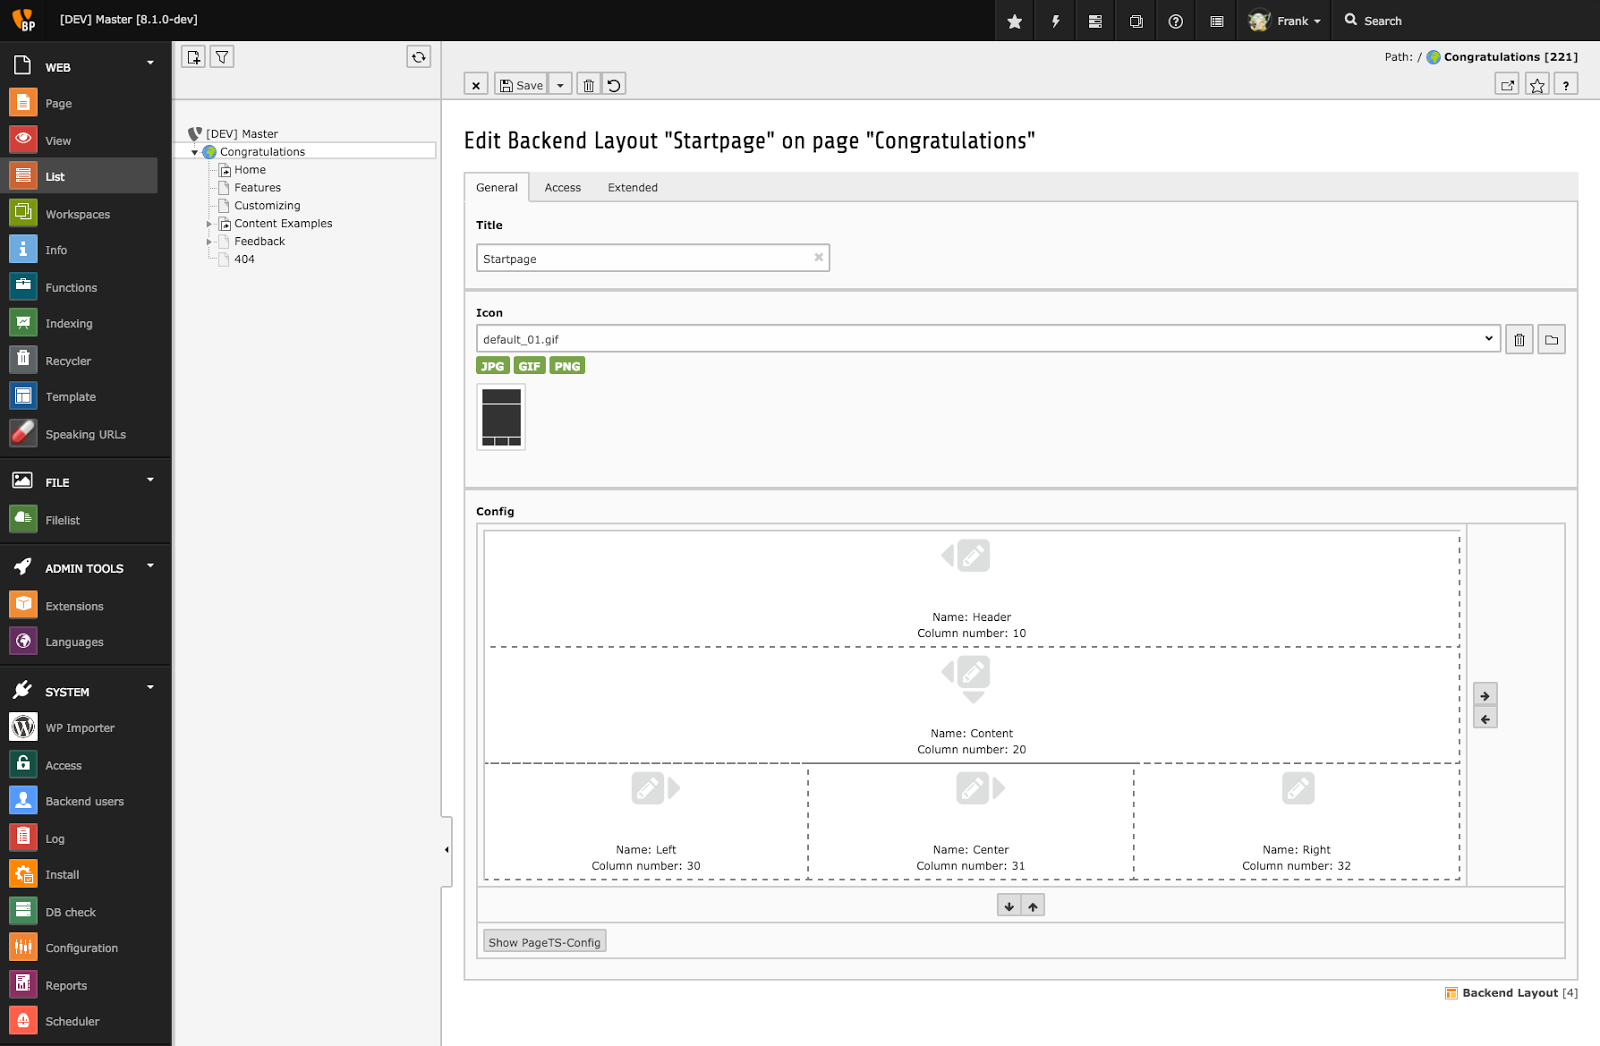
\includegraphics[width=16cm]{Bilder/Typo3_Backend.png}
\caption{Typo3 Backend im Seitenbearbeitungs Modus \cite{Typo3Bild}}
\label{Typo3_Backend_Bild}
\centering
\end{figure}

Es ist m�glich unter Verwendung von PHP, Extbase und Fluid eigene Erweiterungen f�r den Portalserver zu entwickeln. Die jeweiligen Erweiterungen wirken im Fronten von Typo3 wie ganz normale Webseiten.
Auf Extbase und Fluid wird im Kapitel \ref{Typo3} genauer eingegangen.

Ein Vorteil von Typo3 ist, dass es eines der am h�ufigsten verbreiteten Portalserver auf dem Markt ist. Selbst gro�e Firmen wie "`Sixt"' setzten auf Typo3 bei der Erstellung ihrer Internetportale.
Durch die gro�e Verbreitung von Typo3 ist auch die Community um die Software sehr gro� und man findest schell zu fast jedem Problem im Internet eine L�sung.

Typo3 kann im Zusammenspiel mit MySQL, MariaDB, PostgreSQL oder Oracle als Datenbank betrieben werden. Nur mit Hilfe einer dieser Datenbank im Hintergrund ist Typo3 stabil Lauff�hing und kann produktiv eingesetzt werden.

Durch ein �bersichtliches Backend (siehe Abbildung \ref{Typo3_Backend_Bild}), ist es auf f�r Laien m�glich qualitativ Hochwertige Webseiten zu erstellen, ohne viel Kenntnis von Webtechnologien wie HTML oder CSS zu haben.

Ein Upload von Dateien f�r den Download beziehungsweise als Seiten-Kontent ist ebenfalls unter Typo3 m�glich. Zus�tzlich dazu ist es m�glich das Nutzer Dateien auf den hochladen. 
Hierdurch entsteht auch die M�glichkeit ein Austauschportal f�r Dateien zu schaffen. Nutzer k�nnen so in einer sicheren Umgebung sensible Daten untereinander oder mit Mitarbeitern austauschen.
\cite{LobacherTypo3}

\subsection{Typo3 Neos}
Typo3 Neos ist ein relativ neuer Internetportal Server, welcher 2012 aus dem Wunsch heraus entstand Typo3 zukunftssicher zu gestalten.

Als erkannt wurde, dass eine zukunftssichere Typo3 Entwickung basierend auf dem \ac{MVC}-Prinzip eine koplette Neuimplementierung erfordert wurde der Grundstein f�r Typo3 Neos gelegt.
Neben der Entwickung von Typo3 \ac{CMS} wurde die Entwicklung von Typo3 Neos begonnen. Das Ziel war es, einen Nachfolger f�r Typo3 zu entwickeln. Dies gelang jedoch nicht wie vorgesehen.
\cite{WikiTypo3}

Fr�h wurde festgestellt das sich diese die beiden Projekte in unterschiedliche Richtungen entwickeln. Typo3 Neos ist heute in der Version 2.0 erh�ltlich und hat sich zum Ziel gesetzt Webseiten im gegensatz zu Typo3 live im Frontend zu bearbeiten.
Einfach gesagt ist Typo3 ein Internet-Portalserver welcher auf dem \ac{WYSIWYG}-Prinzip aufbaut. Es ist m�glich Webseiten live oder getrennt vom Livesystem im Frontend zu erstellen. 
Die Frontend-Bearbeitung bingt viele Vorteile f�r die Webseitenerstellung f�r Laien. Diese k�nnen eine Seite direkt bearbeiten und Live nehmen.
\cite{LobacherTypo3}

Neos ist bei weitem nicht so verbreitet wie Typo3 \ac{CMS} und die Community um das Projekt ist deutlich geringer. Dies ist ein klarer Nachteil zum gro�en Bruder Typo3 \ac{CMS} ist.

�hnlich wie bei Typo3 \ac{CMS} ist es in Neos m�glich sogenannte Plugins zu entwickeln. Diese basieren auf dem "`Typo3 Flow"'-Framework, welche zusammen mit Neos entwickelt wurde.
Flow ist ein Framework, welches es erlaubt Templates mit Hilfe von "`Fluid"' zu entwickeln. Auf die Fluid wird im Abschnitt \ref{Fluid} n�her eingegangen.
\cite{WikiFlow}

�hnlich wie Typo3 \ac{CMS} ben�tigt auch Neos eine SQL-Datenbank zur Datenhaltung und ist Quelloffen verf�gbar. Nach der Abspaltung von Typo3 Neos vom Typo3 Projekt, wird es heute von einer relativ kleinen Gemeinde entwickelt.
Aus diesem Grund, gibt es keine Roadmap f�r das Projekt und die Ver�ffentlichung von neuen Version ist tr�ger als die von Typo3 \ac{CMS}. 

\begin{figure}[!ht]
\centering
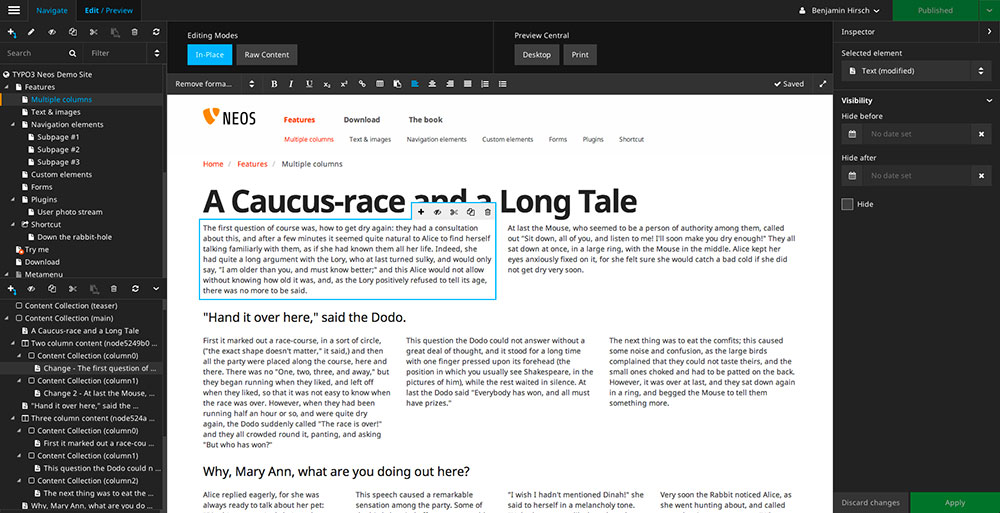
\includegraphics[width=16cm]{Bilder/neos_backend.jpg}
\caption{Typo3 Neos Backend im Seitenbearbeitungs Modus \cite{NeosBild}}
\label{Typo3_Neos_Backend_Bild}
\centering
\end{figure}

In Abbildung \ref{Typo3_Neos_Backend_Bild} ist der Seitenbearbeitungs-Modus von Neos zu sehen. Es ist gut zu erkennen, das Inhalte einer Webseite direkt bearbeitet werden k�nnen. Dies macht eine Webentwicklung f�r Laien einfacher.
\subsection{Joomla}
Joomla ist ein weiteres \ac{CMS}-System f�r die Erstellung von Webseiten. �hnlich wie Typo3 ist es Open Source und nutzt eine MySQL-Datenbank im Hintergrund. Das System ist in PHP5 geschrieben und dient in erster Linie zur Erstellung von Webseiten.
Am besten kann Joomla mit Typo3 Neos verglichen werden, da es einen �hnlichen Ansatz zur Erstellung von Webseiten aufgreift. 

Ein Vorteil gegen�ber Neos ist, das Joomla weit verbreitet ist und eine beachtliche Community hat, welche bei Neos geringer ausf�llt. Nachteilig an Neos ist jedoch, das es eine Bearbeitung von Web-Inhalten nur im Backend zul�sst. Dies bedeutet wiederum, das mehr Erfahrung ben�tigt wird um eine Webseite zu erstellen.

Weitere Nachteile sind zum einen die kaum existente Roadmap, welche zur Zeit der Bearbeitung nicht aktuell war. Zum anderen ist die Entwicklung von Erweiterungen f�r Joomla nicht so gut strukturiert wie es bei Typo3 mit Fluid der Fall ist.

Eine freie Gestalltung der Webseiten ist zwar gegeben, aber f�r die Entwicklung eines komplexes Supportportals wie es sp�ter einmal entstehen soll ist Joomla nicht oder nur bedingt geeignet.
Es gibt momentan keine garantierte Weiterentwicklung des Portalservers und eine Unterst�tzung von MariaDB ist nicht offiziell gegeben.

Auch wenn Joomla durchaus seinen Charm hat, so ist es f�r die Entwicklung eines Supportportals, welches modular aufgebaut werden soll nicht zu empfehlen. Dies bedingt sich zum einen aus der abgelaufen Roadmap, aber auch durch die schlechtere Erweiterungsentwicklung im Gegensatz zu Typo3 \ac{CMS} oder Neos.
\subsection{Drupal}
\subsection{Auswertung der m�glichkeiten}
Auch wenn Typo3 Neos Typo3 \ac{CMS} in nichts nachsteht, so wurde sich dennoch gegen die Verwendung von Neos entschieden, da eine vorranscchreitende Entwicklung nicht gewehrleistet. 
Im Punkto Zukunftssicherheit ist Typo3 \ac{CMS} deutlich besser aufgestellt. 

\newpage
\section{Typo3}\label{Typo3}
Im Abschnitt \ref{PortalServerTypo3} wurde schon grundlegend auf Typo3 eingegangen. Es stellte sich im Abschnitt \ref{PortalserverAuswertung} heraus, dass Typo3 die besten M�glichkeiten bietet um ein modulares Supportsystem aufzubauen.

Im folgenden Kapitel wird genauer auf die Verwendung von Typo3 \ac{CMS} (im weiteren als Typo3 bezeichnet) eingegangen.
Hierbei wird auf die Roadmap von Typo3 eingegangen und gezeigt wie eine Typo3 Extension grundlegend entwickelt wird.

\subsection{Typo3 8.5}
Die momentan aktuelle \ac{LTS}-Version von Typo3 ist die Version 7, welche aktuell (Stand Dezember 2016) noch immer unterst�tzt wird.
Gleichzeitg wird eine neue \ac{LTS}-Version entwickelt, welche iterativ innerhalb der Version 8.x entsteht. Momentan ist die aktuelle Version 8.5, welche zum Beispiel einen neuen \ac{RTE}-Editor mitbringt. \cite{Typo85}

Im Verlauf des Jahres 2017, soll dann die neue \ac{LTS}-Version von Typo3 erscheinen. Da sich die Entwicklung des Supportportals vorraussichtlich bis Ende 2017 erstrecken wird, ist es nur logisch die Neuentwicklung auf den momentanen Zwischenversionen zu entwickeln, um bei der Fertigstellung m�glichst auf einer neuen \ac{LTS}-Version aufsetzen zu k�nnen.

\subsection{Extensions}
Es ist m�glich beinahe jede ben�tigte Funktion in Typo3 einzubauen. Dies geschieht �ber so genannte Extensions, welche den Funktionsumfang von Typo3 erweitern oder ver�ndern k�nnen.
Das Grundsystem, welches nach der Installation vorzufinden ist, basiert zum Teil schon auf Extensions, den sogenannten System-Extensions. Diese Extensions bringen grundlegende Funktionalit�ten in das Grundsystem ein und erweitern dieses. 

Das Auslagern von Funktionalit�ten in Extensions hat mehrere Vorteile. Zum einen entlastet es den System-Kern und macht diesen schlanker und �bersichtlicher. Zum anderen k�nnen Fehler in Extensions behoben werden, ohne das ganze System zu updaten. 

Konzepte von Typo3 Extensions sind zum einen die objektorienterte Programmierung und das \ac{MVC}-Prinzip.

\newpage
\paragraph{Objektorienterte Programmierung} sagt aus, dass alles und jedes im Programm auf Klassen basiert. Lediglich PHP-Funktionalit�ten wie finale Klassen oder die Sichtbarkeit "`private"' wird nicht unterst�tzt. 

Der gesammte PHP-Quellcode einer Extension ist Objektbasiert, nicht nur Modellklassen, sondern auch Konstroller oder Repositorys sind als Klassen abgebildet. 

\begin{wrapfigure}{r}{4cm}
\centering
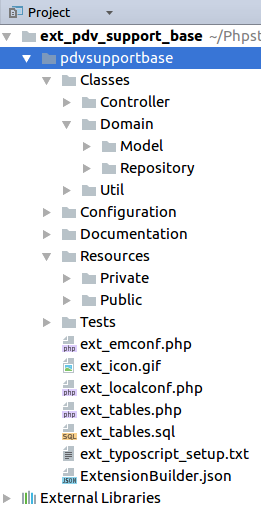
\includegraphics[width=4cm]{Bilder/projekt_struktur.png}
\caption{Extension Struktur}
\label{Extension Struktur}
\vspace{-80pt}
\end{wrapfigure}

\paragraph{Model-View-Controller}\label{MVCTypo} ist ein sehr bekanntes Strukturierungsmittel in der Informatik und kommt auch bei Typo3 Extensions zum Einsatz.
In einem Extension-Projekt, m�ssen alle Klassen innerhalb fester Pfade abgelegt werden.

In Abbildung \ref{Extension Struktur} ist die Struktur der Basis-Extension f�r das Supportportal zu sehen.

\subparagraph{Modellklassen,} welche nach dem \ac{MVC}-Prinzip reale Objekte verk�rpern, sind unter Classes/Domain/Model zu finden.
\subparagraph{Controller} sind unter Classes/Controller zu finden.
\subparagraph{Views,} welche bei Webseiten als HTML-Dateien realisiert werden, sind unter Resources/Private zu finden. Hier wiederum sind sie im Unterordner Templates zu finden. Eine Besonderheit bei Extensions ist, dass wiederkehrende Views so genannte "`Partials"' im Unterordner Partials zu finden sind. Partials werden innerhalb von Templates gerendert und dargsestellt.

Eine weitere Besonderheit sind die Repository-Klassen, welche unter /Classes/Domain/Repository zu finden sind. Sie stellen die Persistenzschicht zwischen Anwendung und Datenbank dar. Alle Lese- oder Schreiboperationen werden innerhalb der Repositorys durchgef�hrt. Typo3 stellt innerhalb der Repositorys viele dynamische Methode bereit, um Standardabfrage zu realisieren.

Um den Grundstock f�r eine neue eigene Extension zu legen, kann der Extension-Builder\footnote{\url{https://typo3.org/extensions/repository/view/extension_builder}} verwendet werden. Dieser baut unter Angabe des Domain-Modells und der Constroller die Grundextension auf, die dann mit Inhalt gef�llt werden kann.

Eine genauere Beschreibung, aller Komponenten einer Extension und wie eine Extension grundlegend zu Programmieren ist, kann in den B�chern von Patrick Lobacher\footnote{Typo3 Extbase} nachgelesen werden. Lobacher beschreibt in verschiedenen B�chern die Grundlagen f�r die Programmierung anhand verschiedener Typo3 Versionen.

\subsection{TypoScript}
TypoScript ist eine eigens f�r Typo3 entwickelte Konfigurationssprache mit der es m�glich ist, eine Typo3 Extension zu konfigurieren.
Eine Sprachdefinition zu TypoScript findet sich in der TypoScript Reference\footnote{\url{https://docs.typo3.org/typo3cms/TyposcriptReference/}}.

Das eigentliche TypoScript f�r jede Extension ist unter Configuration/TypoScript (siehe Abbildung \ref{Extension Struktur}) in der Datei setup.txt zu finden.
Zus�tzlich zu der Konfiguration findet sich im selben Ordner noch eine Datei constants.txt, in welcher globale Konstanten f�r die Extension definiert werden k�nnen. \cite{TypoScript}

Konstanten, welche in der constants.txt, zu finden sind, k�nnen aber zus�tzlich innerhalb von Typo3 ge�ndert werden. Dies bietet bei richtiger Programmierung einer Extension eine gro�e Flexibilit�t. Zum Beispiel k�nnen in einer, entsprechend zur vorliegenden Arbeit, entwickelten Extension �ber Konstanten verschiedene Dinge angepasst werden. Es ist so m�glich ohne Eingriff in den Quellcode, Links im Footer der Extension zu �ndern. (Mehr zu entwickelten Extension siehe Kapitel \ref{Modulare Extensions})

Wie genau Extension mit Hilfe von TypoScript konfiguriert werden k�nnen, ist in der offizellen Dokumentation oder in den B�chern von Patrick Lobacher genauer beschrieben.

\subsection{Fluid}\label{Fluid}
Fluid ist eine Typo3 System Extension, welche ein Framework f�r das Rendern von Templates bereit stellt. Zu jeder Aktion, welche es innerhalb eines Controllers (siehe \ref{MVCTypo}) gibt existiert auch ein Fluid Template, sofern kein Redirect zu einer anderen Aktion durchgef�hrt wird. 

Hat die Aktion des Controllers alle f�r das Template ben�tigten Daten ermittelt, so werden diese Fluid �bergeben. Fluid wiederum bestimmt anhand der Namen des Controllers und der Aktion, das jeweilige Template und rendert es mit den entsprechenden Daten. 

Fluid ermittelt das entsprechende Template wie folgt Resources/Private/Templates/<<Controller Name>>/<<Aktion Name>>.html.

Innerhalb eines Template k�nnen verschiedene Partials angegeben sein, welche wiederkehrende Teile enthalten (siehe \ref{MVCTypo}). 

Was Fluid jedoch so m�chtig macht, sind die sogenannten "`ViewHelper"'. ViewHelper sind Tags, welche Fluid anweisen, PHP-Routinen auszuf�hren. Diesen PHP-Routinen k�nnen f�r ihrere Arbeit Daten �bergeben werden und geben an Fluid, dass entsprechende Ergebnis zur�ck, welches dann wiederum im Template durch den eigentlichen ViewHelper-Tag ersetzt wird.

\lstinputlisting[language=html, caption=Beispiel f�r ein ViewHelper, label=template example, captionpos=b]{Code/template_example.html}

Im HTML-Beispiel \ref{template example} ist ein Ausschnitt aus einem Template zu sehen, welcher einen ViewHelper f�r eine For-Schleife zeigt.
Beim rendern des Templates, wird f�r jeden Eintrag innerhalb von "`{tempUsers}"' der Inhalt des Tags f:for dupliziert. Zus�tzlich ersetzt Fluid die Platzhalter in den geschweiften Klammern mit den realen Werten.

\subsection{Schematische Darstellung eines Seitenaufrufs}
In den vorangegangen Abschnitten wurden die einzelnen Bestandteile und der interne Aufbau einer Typo3 Extension beschrieben. Zur besseren Verdeutlichung des Seitenaufrufs einer Typo3 Extension, stellt die Abbildung \ref{Typo3_Call} den Zusammenhang noch einmal dar.

\begin{figure}[!ht]
\centering
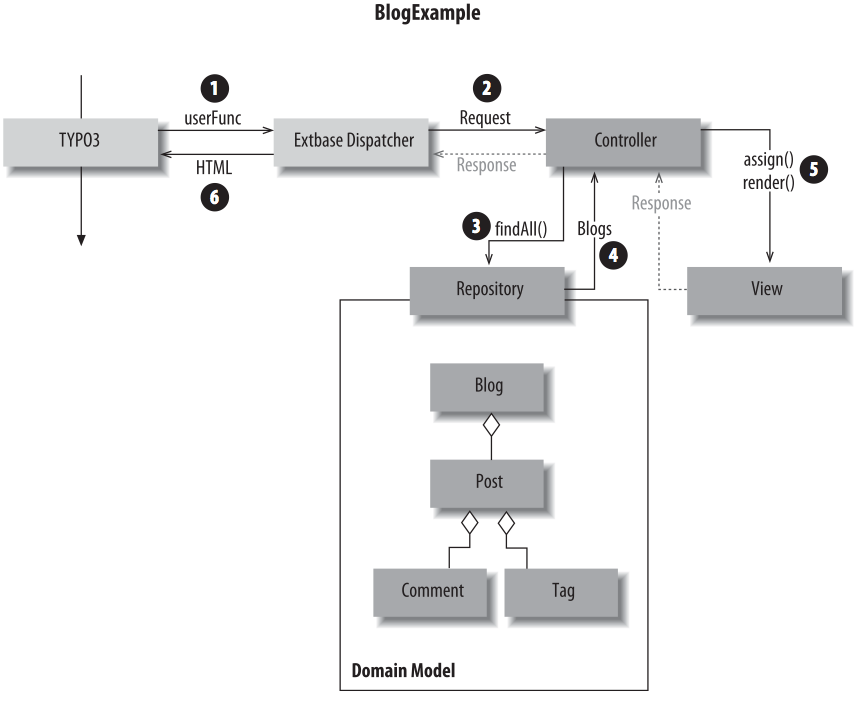
\includegraphics[width=12cm]{Bilder/typo3_aufruf.png}
\caption{Seitenaufruf einer Typo3 Extension\cite{Typo3Call}}
\label{Typo3_Call}
\centering
\end{figure}

\FloatBarrier

\begin{enumerate}
 \item Nutzer ruft eine Funktion auf 
 \item Extbase Dispatcher leitet Request an entsprechenden Controller/ Aktion
 \item Aktion nutzt Repositorys um Daten zu suchen
 \item Repository liefert Daten zur�ck
 \item Aktion ruft den View (Fluid) auf und �bergibt die Daten
 \item Fluid rendert das Template mit den Daten und gibt das HTML zur�ck
\end{enumerate}

\newpage
\section{Modulare Extensions}\label{Modulare Extensions}
Im im Folgenden soll evaluiert werden in wie weit es m�glich ist, dass verschiedene Extensions zusammen arbeiten k�nnen.
Das Supportportal im Ganzen soll aus verschiedenen Extensions bestehen, welche modular auf einander aufbauen. 

Es sollen folgende Extensions erstellt werden:

\FloatBarrier
\begin{minipage}{3cm}
\textit{Template}
\end{minipage}
\begin{minipage}{13cm}
In der \textit{Template} Extension wird das grundlegende Layout des Supportportals definiert.\\
Zus�tzlich kommen noch einige ViewHelper und Utility-Funktion hinzu, welche von mehreren anderen Extensions genutzt werden k�nnen.\\
Alle anderen Extensions bauen auf dieser auf und sind ohne diese nicht Lauff�hig.\\
\end{minipage}

\begin{minipage}{3cm}
\textit{SupportBase}
\end{minipage}
\begin{minipage}{13cm}
Die Extension \textit{SupportBase} stellt das grundlegende Datenmodell zur Verf�gung, das andere Extensions nutzen und auch erweitern k�nnen.\\
Zus�tzlich k�mmert sich diese Extension auch um das Login der Nutzer. Dies schlie�t die Neuanmeldung und das �ndern des Passwortes mit ein.\\
\end{minipage}

\begin{minipage}{3cm}
\textit{Polymer}
\end{minipage}
\begin{minipage}{13cm}
Die \textit{Polymer}-Extension stellt \textit{Polymer}-Elemente (siehe Abschnitt \ref{Typo und Polymer}) in Form von ViewHelpern (siehe Abschnitt \ref{Fluid}) zur Verf�gung. Sie bildet eine Sammlung von \textit{Polymer}-Elementen, welche andere Extensions verwenden k�nnen.\\
Alle Extensions, welche \textit{Polymer}-Elemente verwenden, sind von ihr abh�ngig.\\
\end{minipage}

\begin{minipage}{3cm}
\textit{DownloadPortal}
\end{minipage}
\begin{minipage}{13cm}
Die Extension erweitert das Datenmodell der \textit{SupportBase} und stellt f�r die Nutzer von PDV-Produkten wichtige Downloads bereit.\\
Zus�tzlich bietet sie eine Abo-Funkion an, in der Nutzer sich f�r bestimmte Download-Kategorien anmelden k�nnen. Bei neuen Downloads werden sie dann entsprechend benachrichtigt.\\
\end{minipage}

\begin{minipage}{3cm}
\textit{SupportPortal}
\end{minipage}
\begin{minipage}{13cm}
Die \textit{SupportPortal}-Extension ist das Herzst�ck des allumfassenden Supportportals. Mit ihr ist es m�glich Calls zu Problemen oder Software-Bugs zu �ffenen und mit Supportmitarbeitern in Kontakt zu treten.\\
\end{minipage}

\begin{minipage}{3cm}
\textit{KnowledgeBase}
\end{minipage}
\begin{minipage}{13cm}
Die \textit{KnowledgeBase} ist, wie der Name schon sagt, ein Verzeichnis mit bekannten Problemen und Hinweisen zum verwenden der PDV-Software. Sie bezieht sich auf Daten aus der \textit{SupportBase}.\\
\end{minipage}

\begin{minipage}{3cm}
\textit{DataExchange}
\end{minipage}
\begin{minipage}{13cm}
Um den Datenaustaus zwischen Kunden zu gew�hrleisten, soll die Extension \textit{DataExchange} geschaffen werden. �ber sie ist es m�glich, dass PDV-Mitarbeiter Kunden Daten zur Verf�gung stellen und umgekehrt.\\
\end{minipage}

\begin{minipage}{3cm}
\textit{AdminSchulung}
\end{minipage}
\begin{minipage}{13cm}
Die \textit{AdminSchulung} ist eine Extension, welche es der PDV Systeme GmbH erlaubt Schulungen und Pr�fungen f�r Systemadministratoren online durchf�hren zu k�nnen.\\
\end{minipage}

Die Extensions \textit{Template}, \textit{SupportBase} und \textit{Polymer} stellen grundlegende Extensions dar, von denen alle Support-Extensions abh�ngig sind. Die Support-Extensions \textit{DownloadPortal}, \textit{SupportPortal}, \textit{KnowledgeBase}, \textit{DataExchange} und \textit{AdminSchulung} sind alle voneinander unabh�nig und k�nnen modular eingesetzt werden.

Innerhalb der vorliegenden Arbeit sollen nicht alle Extensions programmiert werden, da dies aus Gr�nden des Aufwandes nicht m�glich ist. Es soll lediglich Anhand der Extensions \textit{Template}, \textit{Polymer}, \textit{SupportBase} und \textit{DownloadPortal} gezeigt werden, dass modulare Extensions unter Typo3 m�glich sind und wie ein L�sungsansatz aussehen kann.

Im weiteren Verlauf wird ebenso auf die genaue Programmierung der einzelnen Extensions verzichtet. Es wird sich auf die Schwerpunkte bezogen, welche wichtig sind um die Extensions modular aufzubauen und wie es m�glich ist, moderne Web-Technologien wie \textit{Polymer} oder AngularJS in Typo3 Extensions einzubauen (siehe Kapitel \ref{Zusammenspiel der Technologien}).

\subsection{Datenbasis}
\subsection{Rendering}\label{Rendering}
Im folgenden Abschnitt, soll dargestellt werden, wie es unter TYPO3 m�glich ist ein modulares Rendering aufzubauen. 
Dies geschieht am Beispiel der oberen Men�leiste des des Templates.

Die \textit{Template}-Extension stellt die grundlegende Men�leiste siehe Abbildung ????? dar.
Ohne eine Extension, welche das Login bereitstellt (\textit{SupportBase}), kann die \textit{Template}-Extension also keinen Login darstellen.
Alle Elemente wie zum Beispiel Buttons, welche modale Dialoge zum Einloggen triggern, m�ssen also bei rendern vom Template gesucht und eingebunden werden. Dies betrifft nat�rlich auch die modalen Dialoge selbst.

Um das eben beschriebene Problemen zu l�sen, wurde ein \textit{ViewHelper} entwickelt, welcher innerhalb der Men�leiste eingebunden werden kann.
Wird nun das Template mit der Men�leiste gerendert, wird der \textit{ViewHelper} aufgerufen, welcher die entsprechend Elemente in die Men�leiste rendert.

Der \textit{ViewHelper} muss nun alle installierten Extensions nach Elementen durchsuchen, welche innerhalb der Men�leiste gerendert werden sollen. Hierbei muss nat�rlich darauf geachtet werden, dass es in der Men�leiste drei Arten von Elementen gibt. 

\begin{itemize}
 \item Elemente die immer geladen werden m�ssen
 \item Elemente die angezeigt werden, wenn der Nutzer eingeloggt ist
 \item Elemente die angezeigt werden, wenn der Nutzer nicht eingeloggt ist
\end{itemize}

Damit die entsprechenden Elemente gefunden und im passenden Fall geladen werden, wurden drei Annotationen geschaffen, mit denen die entsprechenden HTML-Dateien beginnen m�ssen.

\begin{itemize}
 \item \texttt{@additionHTML}
 \item \texttt{@authenticated}
 \item \texttt{@notAuthenticated}
\end{itemize}

Um die Suche nach entsprechenden HTML-Dateien zu beschleunigen, wurde festgelegt, dass Elemente nur in Extensions gesucht werden, welche mit "`pdv"' beginnen. Somit durchsucht der ViewHelper nur PDV eigene Extensions, welche nach der Konvention mit "`pdv"' beginnen. Damit die Suche noch schneller von statten geht, wurde au�erdem festgelegt, dass Elemente innerhalb eines festgelegt Pfades zu finden sind. Konkret bedeutet das, dass Elemente innerhalb von Extensions im Pfad \texttt{Resources/Private/NavBar} abgelegt werden m�ssen.

Damit der \textit{ViewHelper} die entsprechenden Element-Arten an den richtigen stellen einbringt, kann dieser mit Hilfe des Attributs \textit{section} gesteuert werden.

\begin{itemize}
 \item \texttt{add}
 \item \texttt{Auth}
 \item \texttt{noAuth}
\end{itemize}

\lstinputlisting[language=html, caption=ViewHelper-Aufruf, label=NavViewHelper, captionpos=b]{Code/nav_helper.html}

Im Codebeispiel \ref{NavViewHelper} wird der Aufruf des \textit{ViewHelpers} schematisch dargestellt. �ber den \textit{Standard-ViewHelper} \texttt{ifAuthenticated} gepr�ft, ob der Nutzer angemeldet ist. Ist dies der Fall, wird wiederum der eben beschriebene \texttt{NavBarViewHelper} mit dem Attribut \texttt{section="\ Auth"} aufgerufen. Somit sucht der \textit{ViewHelper} beim Rendern nun nach allen Elementen, die angezeigt werden m�ssen wenn ein Nutzer angemeldet ist.

\begin{figure}[!ht]
\centering
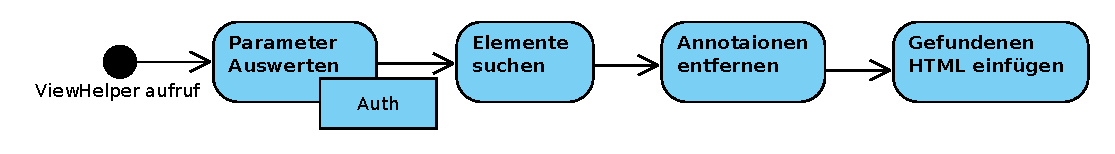
\includegraphics[width=16cm]{Bilder/NavBar.eps}
\caption{Darstellung des NavBarViewHelper}
\label{NavBarViewHelper}
\centering
\end{figure}

In Abbildung \ref{NavBarViewHelper} ist die Funkion des \texttt{NavBarViewHelper} noch einmal schematisch dargestellt. Der \textit{ViewHelper} wird mit einem Parameter aufgerufen. Dieser wird zuerst ausgewertet, um zu bestimmen, welche Elemente ben�tigt werden. Anschliesend werden im n�chsten Schritt die entsprechenden Elemente gesucht. Als n�chstes, wird die Annotationen aus den geladenen HTML-Elementen entfernt. Zum Schluss werden alle geladenen Elemente anstelle des \textit{ViewHelpers} innerhalb das angeforderten HTML-Template eingef�gt.

TYPO3 besitzt sehr intelligente Caching-Mechanismen die ein solches vorgehen erlauben. Denn durch die Nutzung von Caches erstellt TYPO3 nicht bei jedem Seitenaufruf das Template neu.

% TYPO3 unterst�tzt war "`Partials"', welche Teil-Templates innerhalb von Templates darstellen, diese k�nnen aber nicht dynamisch geladen werden.
\newpage
\section{Neue Webtechnologien}
\subsection{Google Polymer}\label{Google Polymer}
Polymer Einleitung!
\subsubsection{Wozu Polymer Elemente}\label{Wozu Polymer Elemente}
Polymer Elemente versuchen so genannten Boiler-Code zu vermeiden. Als Boiler-Code wird die Verschmelzung verschiedener Programmiersprachen innerhalb einer Datei oder eines Elements bezeichnet. Boiler-Code ist h�ufig in Web-Seiten zu finden. 

Um eine HTML-Element zu erstellen wird als Grundger�st HTML verwendet. Zus�tzlich enth�lt das HTML-Element aber auch CSS um das aussehen zu beeinflussen. Um ein HTML-Element dynamisch oder interaktiv zu gestalten wird meist zus�tzlich auch noch Java-Skript oder AngularJS verwendet. Typischer weise findet mal alle drei Sprachen in einer HTML-Datei oder in getrennten Dateien. 

Jedoch haben beide Ans�tze Nachteile. Bei der Vereinigung verschiedener Sprachen in einer Datei, leidet meist die �bersicht, denn CSS, Java-Skript und zugeh�riges HTML muss nicht an festen Positionen sein. So kommt es �fter vor, dass zusammengeh�rige Elemente innerhalb einer Datei weit auseinander stehen.

Der Ansatz die verschiedenen Sprachen zu trennen, beseitigt zwar das durcheinander innerhalb der HTML-Dateien, jedoch entstehen hier wieder neue Probleme. Wenn alle Sprachen strikt in verschiedenen Dateien sind, ist es oft nur schwer nachzuvollziehen, welches Java-Skript zu welchem HTML-Element geh�rt. F�r au�enstehende Programmiere ist dies oft eine unl�sbare Aufgabe.

\subsubsection{Was macht Polymer aus}
Polymer wiederum geht, im Gegensatz zu den beiden im Abschnitt \ref{Wozu Polymer Elemente} genannten, einen dritten sehr eleganten Ansatz. Grunds�tzlich kommen bei Polymer verschiedene Programmiersprachen und Konzepte wieder zusammen in eine HTML-Datei. 

Der entscheidende Unterschied jedoch ist, das HTML, CSS und Skripte ihre festen Bereiche haben, in denen sie implementiert werden. Dies gestaltet die HTML-Datei des jeweiligen Elements sehr �bersichtlich. 

Ein weiterer Vorteil ist, dass in der Web-Seite, in der das Element Verwendung findet nur noch ein einzelner Tag zu sehen ist, der auf das Polymer Element verweist.

Damit der Polymer das entsprechende Element parsen kann muss vor der Verwendung das jeweilige Element �ber den HTML-Link-Tag eingebunden werden.

\subsubsection{Ein eigenes Polymer Element erstellen}\label{Ein eigenes Polymer Element erstellen}
Um zu zeigen, wie einfach es ist auf Basis von Polymer Elemente selbst zu erstellen folgt in den nun kommenden Abschnitten nun Beispiel, welches im Kapitel \ref{Zusammenspiel der Technologien} in Typo3 eingebunden wird.

\lstinputlisting[language=html, caption=Beispiel f�r ein eigenes Polymer-Element, label=Polymer Element, captionpos=b]{Code/polymer_element.html}

Als erstes wird der Polymer-Link hinzugef�gt, welcher immer vorhanden sein muss. Danach folgt der Tag "`dom-module"', welcher die genaue Beschreibung des Elements enth�lt. Im "`template"'-Tag wird das HTML eingef�gt, welches das Element beinhaltet. Hierauf kann optional ein "`style"'-Tag folgen, in welchem der Style des HTML-Elements per CSS angegeben wird. 

\paragraph{CSS f�r ein Element}
Die Definition von CSS hat nur Einfluss auf das jeweilige Template. Elemente au�erhalb des Element-DOM werden von dem hier definiertem CSS nicht beeinflusst.

Es ist jedoch umgekehrt m�glich, CSS-Klassen zu nutzen, im globalen CSS beschrieben sind. Eine erneute Einbindung der CSS-Datei in das Polymer-Element ist nicht notwendig.
Die Verwendung von CSS-Abh�ngigkeiten in Polymer ist jedoch unsch�n, da dies ein Element gegebenen Falls auf Web-Seiten beschr�nkt, welche diese bestimmte CSS-Datei verwenden.
Es ist somit in den meisten F�llen besser keine CSS-Abh�ngigkeiten in Elementen zu verwenden, vor allem dann wenn diese �ffentlich sind.

Im Listing \ref{Polymer Element} wurden CSS-Abh�ngigkeiten zu MaterializeCSS (Abschnitt \ref{MaterializeCSS}) aufgebaut, eine Begr�ndung hierf�r ist im Kapitel/Abschnitt (?????) zu finden.

\paragraph{Element-Script}
Der "`script"'-Tag enth�lt das jeweilige Skript zum Element. Es ist JSON-Notation gehalten und basiert auf Callbacks.

\subparagraph{Die Registrierung} eines Elements steht immer zu begin des Skripts. Dieser Teil muss also immer vorhanden sein, damit das jeweilige Element �berhaupt dargestellt werden kann.

\lstinputlisting[language=html, caption=Polymer-Element Registrierung, label=Element Registrierung, captionpos=b]{Code/element_registration.html}

\subparagraph{Handler} werden in Polymer verwendet um einzelne Skripte aufzurufen. Innerhalb des Handlers kann ein Java-Skript definiert sein, das ausgef�hrt wird, wenn der jeweilige Handler getriggert wird.

\lstinputlisting[language=html, caption=Polymer-Element Handler, label=Element Handler, captionpos=b]{Code/element_handler.html}

Damit ein Handler �berhaupt zum Tragen kommt, muss er innerhalb des HTML-Tags f�r das dass jeweilige Skript sein soll registriert werden.

\lstinputlisting[language=html, caption=Polymer-Element Handler Registration, label=Element Handler Registration, captionpos=b]{Code/element_handler_registration.html}

\subparagraph{Attribute,} welche das Polymer-Element haben soll, m�ssen ebenfalls im Skript definiert werden.

\lstinputlisting[language=html, caption=Polymer-Element Attribute, label=Element Attribute, captionpos=b]{Code/element_attributes.html}

Das Attribut "`owner"' wird im Beispiel als String definiert, und hat den Standardwert "`Daniel"'.
Jedes im Skript definiertes Attribut l�sst sich bei Verwendung des Elements wie ein normales XML-Attribut verwenden. Wird bei Verwendung des Elements das "`owner"'-Attribut nicht angegeben, so ist es "`Daniel"'. 
Um den Inhalt des Attributs im Template zu verwenden, muss es in doppelten geschweiften Klammern aufgerufen werden. So kann zum Beispiel ein B-Tag wie folgt geschrieben werden.

\lstinputlisting[language=html, caption=Polymer-Element Attribute benutzen, label=Element Attribute benutzen, captionpos=b]{Code/element_attributes_use.html}

\subparagraph{Der Aufruf} dieses Polymer-Elements muss wie im Beispiel umgesetzt werden

\subsubsection{Zusammenfassung}
Polymer bietet wie gezeigt wurde eine echte Alternative zum normalen Web-Seiten-Boiler-Code. Durch die Verwendung von Polymer-Elementen entsteht keine nennenswerte Verz�gerung beim parsen einer Web-Seite durch den Browser.
Es bietet sich daher an, bei Neuentwicklungen auf Polymer zu setzen.

Ob und wie eine Intergration von Polymer in Typo3 m�glich ist, wird im Kapitel \ref{Zusammenspiel der Technologien} n�her beschrieben.

\subsection{AngularJS}
\subsection{HTML5}
\subsection{CSS3}
\ac{CSS} ist eine Designsprache f�r HTML und ist deshalb eine der Hauptkomponenten der Webentwicklung. Mit Hilfe von \ac{CSS} ist es m�glich einzelne HTML-Elemente oder Gruppen zu stylen.
Seit der ersten Version die 1993 erschien, wird CSS kontinuirlich weiterentwickelt und ist heute auf praktisch jeder Web-Seite im einsatz.

Auf der Basis von CSS entwickelten sich im laufe der Jahre immer mehr Frameworks, welche einen Designansatz umsetzten und fertige Klassen f�r die Verwendung bereitstellen.
Eines der heute am h�ufigsten anzutreffenden \ac{CSS}-Frameworks ist "`Bootstrap"'.

Innerhalb der PDV Systeme Erfurt wurde beschlossen das neue Supportportal im "`Material Design"' aufzubauen. Als "`Material Design"' werden Gestaltungsrichtlinen von Google bezeichnet, welche angeben wie eine Android-Applikation oder eine mobile Web-Seite f�r Android aussehen sollte.

Das "`Material Design"' ist ein flaches Design, und geht von der Metapher aus, dass der Bildschirm Papier ist. Jedes Element soll sich also wie reales Papier verhalten und auch so aussehen.
Obwohl das Design sehr schlicht gehalten ist, so kann mit viel Farbe gearbeite werden.
\cite{MaterialDesign}

Die nun folgenden Betrachtungen beziehen sich auf die Umsetzung im "`Material Design"'.

\subsubsection{Bootstrap}
Bootstrap ist ein \ac{CSS} Framework, welches von "`Twitter"' entwickelt wird und das unter der "`MIT-Lizenz"' frei erh�ltlich ist. Durch den modularen Ansatz von Bootstrap ist es sehr leicht m�glich das Framework um eigene Style-Anweisungen zu erg�nzen.
\cite{Bootstrap} \cite{WikiBootstrap}

Bootstrap baut auf dem Less-Parser auf. Less ist eine Sprache, die es sich zum Ziel gesetzt hat das schreiben von \ac{CSS} m�glichst einfach und effizient zu machen. Geschriebender Less-Code muss in \ac{CSS} geparst werden.

Das Bootstrap Framework kann entweder direkt als fertiges \ac{CSS}-Framework oder als Less-Code heruntergeladen werden.

Ein Nachteil von Bootstrap ist, dass es nicht leichtgewichtig ist. Zwar kann es sehr gut erweitert werden, dies macht jedoch das Framework auch Schwerf�llig. 
Soll zum Beispiel ein Bootstrap-Template f�r das "`Material Design"' verwendet werden, muss zun�chst das "`standard Framework"' eingebunden werden. Ein Template wie "`Material Design for Bootstrap"' �berschreibt dann nach der Einbindung zum Teil das standard Framework und erg�nzt es um eigene Klassen.
Der Vorteil bei diesem Vorgehen ist ganz klar, dass ein bestehendes Template relativ leicht ausgetauscht werden kann, ohne dass der eigentliche HTML-Code der Web-Seite angepasst werden muss.

Dieser Vorteil wird schnell zum Nachteil, wenn eine Web-Seite erstellt werden soll bei der es auf Geschwindigkeit ankommt. Durch das �berscheiben des standard Frameworks wird zus�tzliche Zeit beim parsen der Web-Seite ben�tigt, was vorallem bei �lteren PCs auff�llt. 
Zus�tzlich steigt der Overhead beim laden einer Seite, da mehr CSS geladen wird, als tats�chlich ben�tigt wird.

Standardm��ig enth�lt Bootstrap zum Beispiel keinen Date-Picker, welcher jedoch in einem Supportportal unerl�sslich ist. Auch "`Bootstrap Material"' enth�lt keinen Date-Picker im "`Material Design"'.
Durch den modularen Aufbau von Bootstrap kann nat�rlich schnell und einfach ein entsprechendendes Template erg�nzt werden. Dies bedeutet aber wieder zus�tzlichen Overhead.
\cite{MaterialBootstrap}
\subsubsection{MaterializeCSS}\label{MaterializeCSS}
Ein anderes Framework, welches die Design-Richtlinien des "`Material Design"' umsetzt ist das noch recht neue Framework "`MaterializeCSS"'. 
MaterializeCSS ist ein eigenst�ndiges Framework, welches versucht alle gegebenen Gestaltungsrichtlinen m�glichst elegant und performat umzusetzen.

Die MaterializeCSS Quellen sind mit \ac{SASS} geschrieben, und m�ssen vor der Verwendung in CSS komiliert werden. Dieses Vorgehen hat meherer Vorteile. So ist es zum einen sehr einfach m�glich das Framework um eigene Style-Objete zu erweitern. Zum anderen hat es den Vorteil, dass die Farbgebung des gesamten Frameworks an einer Stelle zusammen gefasst ist. 
Soll also die Farbgebung ge�ndert werden, so werden in den \ac{SASS}-Quellen des Frameworks die Farben zentral angepasst. Nach einer erneuten kompilierung stehen dann die Farben im gesamten Framework zur Verf�gung.
Ohne dieses Vorgehen m�ssten die entsprechenden Farben an unz�hligen Stellen innerhalb der \ac{CSS}-Datei angepasst werden.
\cite{Materialize}
Ein weitere Vorteil von MaterializeCSS ist, das viele Templates wie ein Date-Picker im "`Material Design"' schon vorhanden sind. Diese Templates k�nnen ohne zus�tzlichen Overhead verwendet werden.

Auch wenn MaterializeCSS noch sehr jung im Vergleich zu Bootstrap ist, so ist es doch eine gute alternative, wenn eine Web-Seite im "`Material Design"' umgesetzt werden soll.
\subsection{PHP7}
\subsection{Google Dart}
\section{Zusammenspiel der Technologien}\label{Zusammenspiel der Technologien}
\subsection{Integration von Polymer in Typo3}
Im Abschnitt \ref{Google Polymer} wurde ausf�hrlicher auf die Verwendung und die Erstellung von Polymer-Elementen eingegangen. Nun soll untersucht werden wie sich Polymer m�glichst elegant in Typo3 integrieren l�sst.

Der beste Weg Polymer-Elemente in Typo3 zu integrieren ist, diese in ViewHelper zu kapseln (Siehe Kapitel ?????). 

Das Ziel ist es also, einen ViewHelper zu erstellen, welcher einen ViewHelper-Tag in einen Polymer-Tag umwandelt.

\begin{wrapfigure}{r}{4cm}
\centering
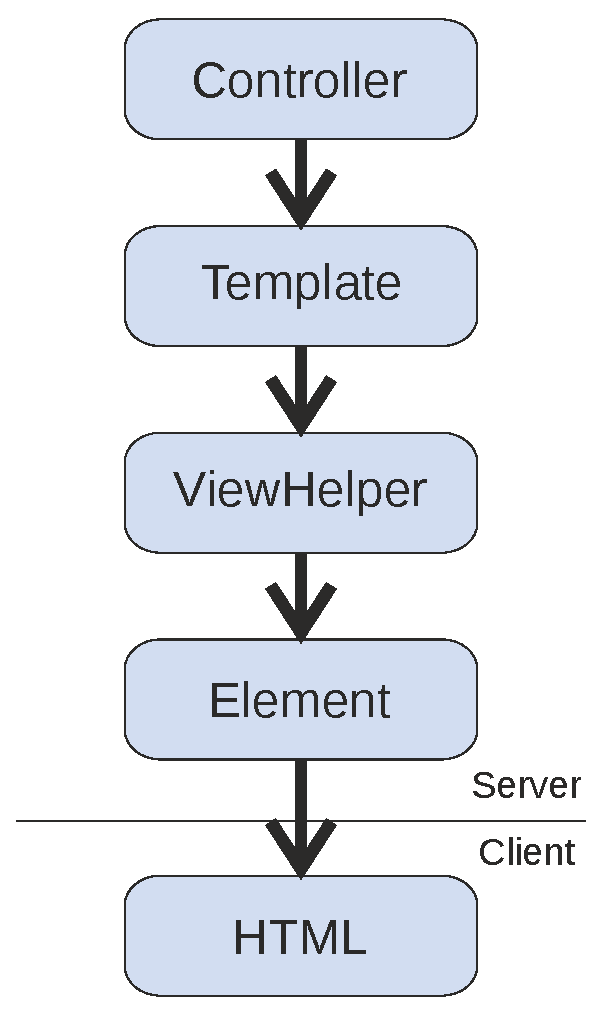
\includegraphics[width=4cm]{Bilder/Polymer.eps}
\caption{Polymer ViewHelper Hirarchie}
\label{Polymer ViewHelper Hirarchie}
\vspace{-40pt}
\end{wrapfigure}

In Abbildung \ref{Polymer ViewHelper Hirarchie} (rechts) ist die Aufrufhirarchie zu sehen, welche innerhalb des Projektes entwickelt wurde, um Polymer Elemente elegant in Typo3 einzuarbeiten.

Die beim laden einer Seite aufgerufene "`Action"' eines bestimmten "`Controllers"' wird aufgerufen. Der "`Controller"' stellt alle zum Rendern des Templates ben�tigte Daten bereit und �bergibt sie dem Template.

Das Template wiederum beinhaltet einen f�r das Polymer Element entwickelten ViewHelper, welcher innerhalb des Templates aufgerufen wird.

Das Fluid-Framework ruft beim Rendern eines Templates den entsprechenden ViewHelper auf. 

Der ViewHelper wiederum gibt den Link zum entsprechenden Polymer Element und den Polymer Tag zur�ck.

Ist das Template fertig gerendert, so wird es an den aufrufenden Client gesendet.

Der Client wiederum ersetzt das Polymer Element durch HTML.

Am Beispiel des Button-Up Elements (siehe Abschnitt \ref{Ein eigenes Polymer Element erstellen}), wird im folgenden erkl�rt, wie dieser Prozess im Quellcode umgesetzt wird.
\newpage
\lstinputlisting[language=php, caption=Polymer ViewHelper, label=Polymer ViewHelper, captionpos=b]{Code/viewhelper.php}

Der ViewHelper erbt von der abstrakten Klasse "`AbstractTagBasedViewHelper"'. Dieser ist in der ViewHelper ist anschlie�end in der Lage, einen HTML-Tag zu ver�ndern.

Mit dem Attribut \$tagname, wird definiert wie der neue Tag hei�en soll, welcher den ViewHelper-Tag ersetzt. Dieser Tag muss nun so hei�en wie das Polymer-Element.

Die Methode "`render"' des ViewHelpers gibt den String zur�ck, der den ViewHelper-Tag ersetzt.

Die "`return"'-Anweisung gibt immer den Link zum entsprechenden Polymer-Element zur�ck, und den Polymer-Tag.

Der ViewHelper wird nun wie folgt aufgerufen.

\lstinputlisting[language=html, caption=Polymer ViewHelper aufrufen, label=Polymer ViewHelper aufrufen, captionpos=b]{Code/viewhelper_call.php}

Beim ausliefern der Web-Seite ersetzt Typo3 nun den ViewHelper-Tag gegen die folgenden HTML-Elemente

\lstinputlisting[language=html, caption=Polymer ViewHelper Ersetzung, label=Polymer ViewHelper Ersetung, captionpos=b]{Code/viewhelper_after.php}

Wird die Web-Seite nun vom Browser gerendert wird, ersetzt er diesen Polymer-Tag schlie�lich durch das definierte Polymer-Element.

Durch die Verwendung von ViewHelpern, kann jedes beliebige Polymer-Element auch unter Typo3 zum Einsatz kommen. Es ist also sehr elegant m�glich Boiler-Code auch in Typo3-Templates und -Partial mit der Hilfe von Polymer zu umgehen.

Durch die Kapselung der Polymer-Elemente in ViewHelpern verhalten sich diese sich au�erdem wie standardm��ige ViewHelper mit Boiler-Code.

Um nun Polymer-Elemente in einem Template zu verwenden, ist kein extra Wissen notwendig, was eine Verwendung so einfach wie m�glich macht. Der Programmierer eines Templates muss sich keine Gedanken �ber Links zu Polymer-Elementen machen und muss sich auch nicht mit Polymer auskennen. Es wird einfach der ViewHelper verwendet und alles andere passiert im Hintergrund.

\subsection{MaterialzeCSS}
Die Integration von MaterializeCSS in Typo3 ist genau so einfach, wie die Integration von Bootstrap oder jedem anderem CSS-Frameworks.
Um MaterializeCSS in Typo3 verwenden zu k�nnen, muss im Template nur angegeben werden, welche CSS-Dateien Typo3 einbinden soll.

Zus�tzlich zu der CSS-Datei ben�tigt MaterializeCSS noch eine eigene Java-Script-Datei und eine aktuelle Version von JQuery. 
Diese Dateien werden zusammen mit dem CSS im Template definiert.

Au�erdem ist es m�glich mit MaterialieCSS die standard Icons und Schriftarten von Google zu nutzen. Sollen dieses Sachen verwendet werden, so m�ssen sie nur zus�tzlich zum CSS und Java-Script im Template definiert werden.

Im Listing \ref{MaterialieCSS Anbindung} ist ein Typo-Script-Beispiel zu sehen, mit welchem MaterializeCSS in Typo3 integriert wird. Das angegebe Typo-Script an entweder in der Konfiguration einer Extension angegeben sein oder es wird direkt in einem Typo3-Template definiert.
\lstinputlisting[caption=MaterialieCSS Anbindung, label=MaterialieCSS Anbindung, captionpos=b]{Code/materilaize_anbindung.txt}
\subsection{Nutzer Anmeldung und Registrierung}

\section{Zusammenfassung}
\section{Fazit}
\newpage
\include{Zusammenspiel_der_Technologien}

\end{spacing}




\newpage
\section{Abk�rzungsverzeichnis}
\begin{acronym}
%   \acro{}{\emph{}}
 \acro{CMS}{\emph{Content Managemente System}}
\acro{LTS}{\emph{Long Term Support}}
\acro{MVC}{\emph{Model View Controller}}
\acro{WYSIWYG}{\emph{What you see is what what you get}}
\acro{CSS}{\emph{Cascading Style Sheets}}
\acro{SASS}{\emph{Syntactically Awesome Stylesheets}}
\acro{MVVM}{\emph{Model View ViewModel}}
\acro{RTE}{\emph{Real Time Editor}}
 %  \acro{GDS}{\emph{Generic Data Services}}
% %  \acro{LSDF}{\emph{Large Scale Data Facility}}
%  \acro{OPM}{\emph{Objektorientierten Programmiermodell}}
%  \acro{SMD}{\emph{Strukturelle Metadaten}}
%  \acro{JSON}{\emph{JavaScript Object Notation}}
% %  \acro{HALO}{\emph{High Altitude and Long Range Research Aircraft}}
%  \acro{IAI}{\emph{Institut f�r Angewandte Informatik}}
%  \acro{JAXB}{\emph{Java Architecture for XML Binding}}
%  \acro{UDDE}{\emph{User Data Description Editor}}
%  \acro{AMD}{\emph{Anwendermetadaten}}
%  \acro{CG}{\emph{Class Generator}}
%  \acro{IG}{\emph{Interface Generator}}
\end{acronym}
\newpage
\listoffigures
\newpage
\listoftables
% Abk�rzungsverzeichnis
\newpage
\bibliographystyle{alpha}
% verzeichnis im DIN format
\bibliography{Quellen}
\end{document}
